
\section{NVLink systems}
NVLink allows for many new possible configurations.
With 4 NVLink ports per Tesla P100 card and 6 per Power8 CPU, and future CPUs with both PCIe and NVLink available, the number of possible configurations is very large.
This design flexibility enables system optimization for different parallel/serial code ratios.
This helps minimizing the impact of Amdahl limits.
In this section come under discussion some of the systems which have already been announced.

\subsection{NVIDIA DGX-1}
In April 2016 the DGX-1 was announced to be produced by Nvidia.
It is recommended by Nvidia for Deep Learning, achieving 170 FP16 TFLOPS in a single node.
It consists of 2 Dual 20-core Intel® Xeon® E5-2698 v4 2.2 GHz and 8 Tesla P100 GPUs.
512GB of DDR4 memory and 128GB of HBM2 memory are available for use as Unified Memory.
Each CPU is connected to 4 GPUs through 2 PCIe switches.
These 2 subsets of 4 GPUs are fully connected through NVLink.
Each subset is also connected through NVLink to the respective GPU of the other subset, as can be seen in Figure \ref{fig:hybrid-cube-mesh}.

\begin{figure}[ht!]
    \centering
    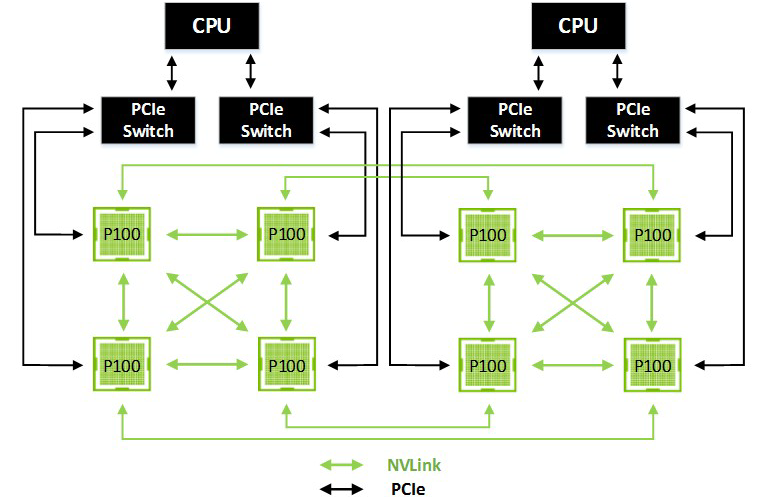
\includegraphics[width=\linewidth]{hybrid-cube-mesh}
    \caption{DGX-1 is connected as a Hybrid Cube Mesh \cite{nvidia:pascalwhitepaper}}
    \label{fig:hybrid-cube-mesh}
\end{figure}

It is expected to provide up to a 12x speed up with respect to the fastest Maxwell node.
The FP16 capability alone accounts for a 2x factor.
Most of the remaining 6x factor is due to increased memory and interconnect bandwidths.


\subsection{NVLink in supercomputing \cite{nvidia:summitsierrawhitepaper}} \label{subsec:nvlsupercomp}
Pushed by the U.S. Department of Energy, the Collaboration of Oak Ridge, Argonne, and Livermore, are planning pre-exascale systems.
Two of them --- Summit and Sierra --- will be based on the OpenPOWER platform, but will have unique system configurations
Both will consist of nodes formed by several Power9 CPUs and several Volta GPUs.
However, only the approximate details of Summit are available and discussed in this section.

Sierra --- managed by the Lawrence Livermore National Laboratory --- will be used for the U.S. nuclear program and counterterrorism.
Sierra will work at at least 100 petaFLOPS.
It will replace Sequoia --- a IBM Blue Gene/Q system --- which was the fastest supercomputer in 2012.

Summit --- managed by the Oak Ridge National Laboratory --- will be used for fundamental scientific research.
Titan --- with 1 GPU per CPU --- is the current top system of ORNL and the 2nd in the TOP500 list.
It is currently oversubscribed.
Summit will perform at 150-300 petaFLOPS, which is about 5-10x of what Titan performs, using only about 10\% additional power.
It will consist of more than 3400 compute nodes, each performing at more than 40 TFLOPS, with 512GB DDR4+HBM and 800GB NVRAM configured as burst buffer or extended memory.
The nodes will be connected as a full non-blocking fat-tree through dual-rail Mellanox EDR Infiniband.
The whole system will use a General Parallel File System with 1TB/s of I/O bandwidth and 120PB of disk capacity.

The key ideas mentioned for the design of both systems are OpenPOWER, NVIDIA Tesla, Heterogeneous Computing and NVLink.
